\section{Strömungsfelder}
\subsection{Stromdichte im Strömungsfeld}
\begin{multicols}{2}
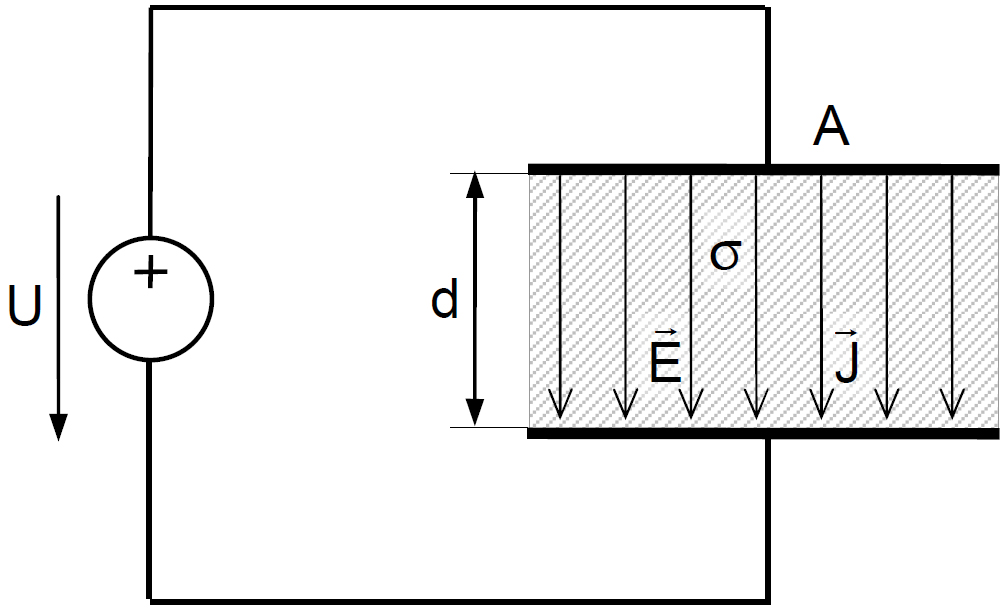
\includegraphics[width=0.3\textwidth]{pics/stroemungsfeld/platten}\\
$ R = \frac{\rho \cdot d}{A} = \frac{d}{\sigma \cdot A}$\\
Leitfähigkeit $ \sigma = \frac{1}{\rho} = \kappa $\\
$ \lbrack \rho \rbrack = \Omega m = \frac{\Omega mm^2}{m} $\\
$ \lbrack \sigma \rbrack = \frac{1}{\Omega m} = \frac{S}{m} $\\
$ I = \frac{U}{R} = \frac{U \cdot \sigma \cdot A}{d} $\\
Stromdichte $ J = \frac{I}{A} = \frac{U \cdot \rho}{d} $\\
$ E = \frac{U}{d} \rightarrow J = \sigma \cdot E $\\
$ \vec J = \sigma \cdot \vec E $ \\
$ \vec E = \rho \cdot \vec J $ \\
\end{multicols}

\subsection{Stromfluss}
\begin{tabular}{ll}
Allgemeiner Fall: & $ I = \int\limits_{A} \vec J \cdot d\vec A $ \\
Falls $ \vec J $ senkrecht auf A steht und J über A konstant ist: & $I = J \cdot A$ \\
Falls das Strömungsfeld homogen und A eine ebene Fläche ist: & $ I = J \cdot A \cdot cos \varphi $
\end{tabular}

\subsection{Potential und Spannung im el. Str"omungsfeld}
\begin{multicols}{2}
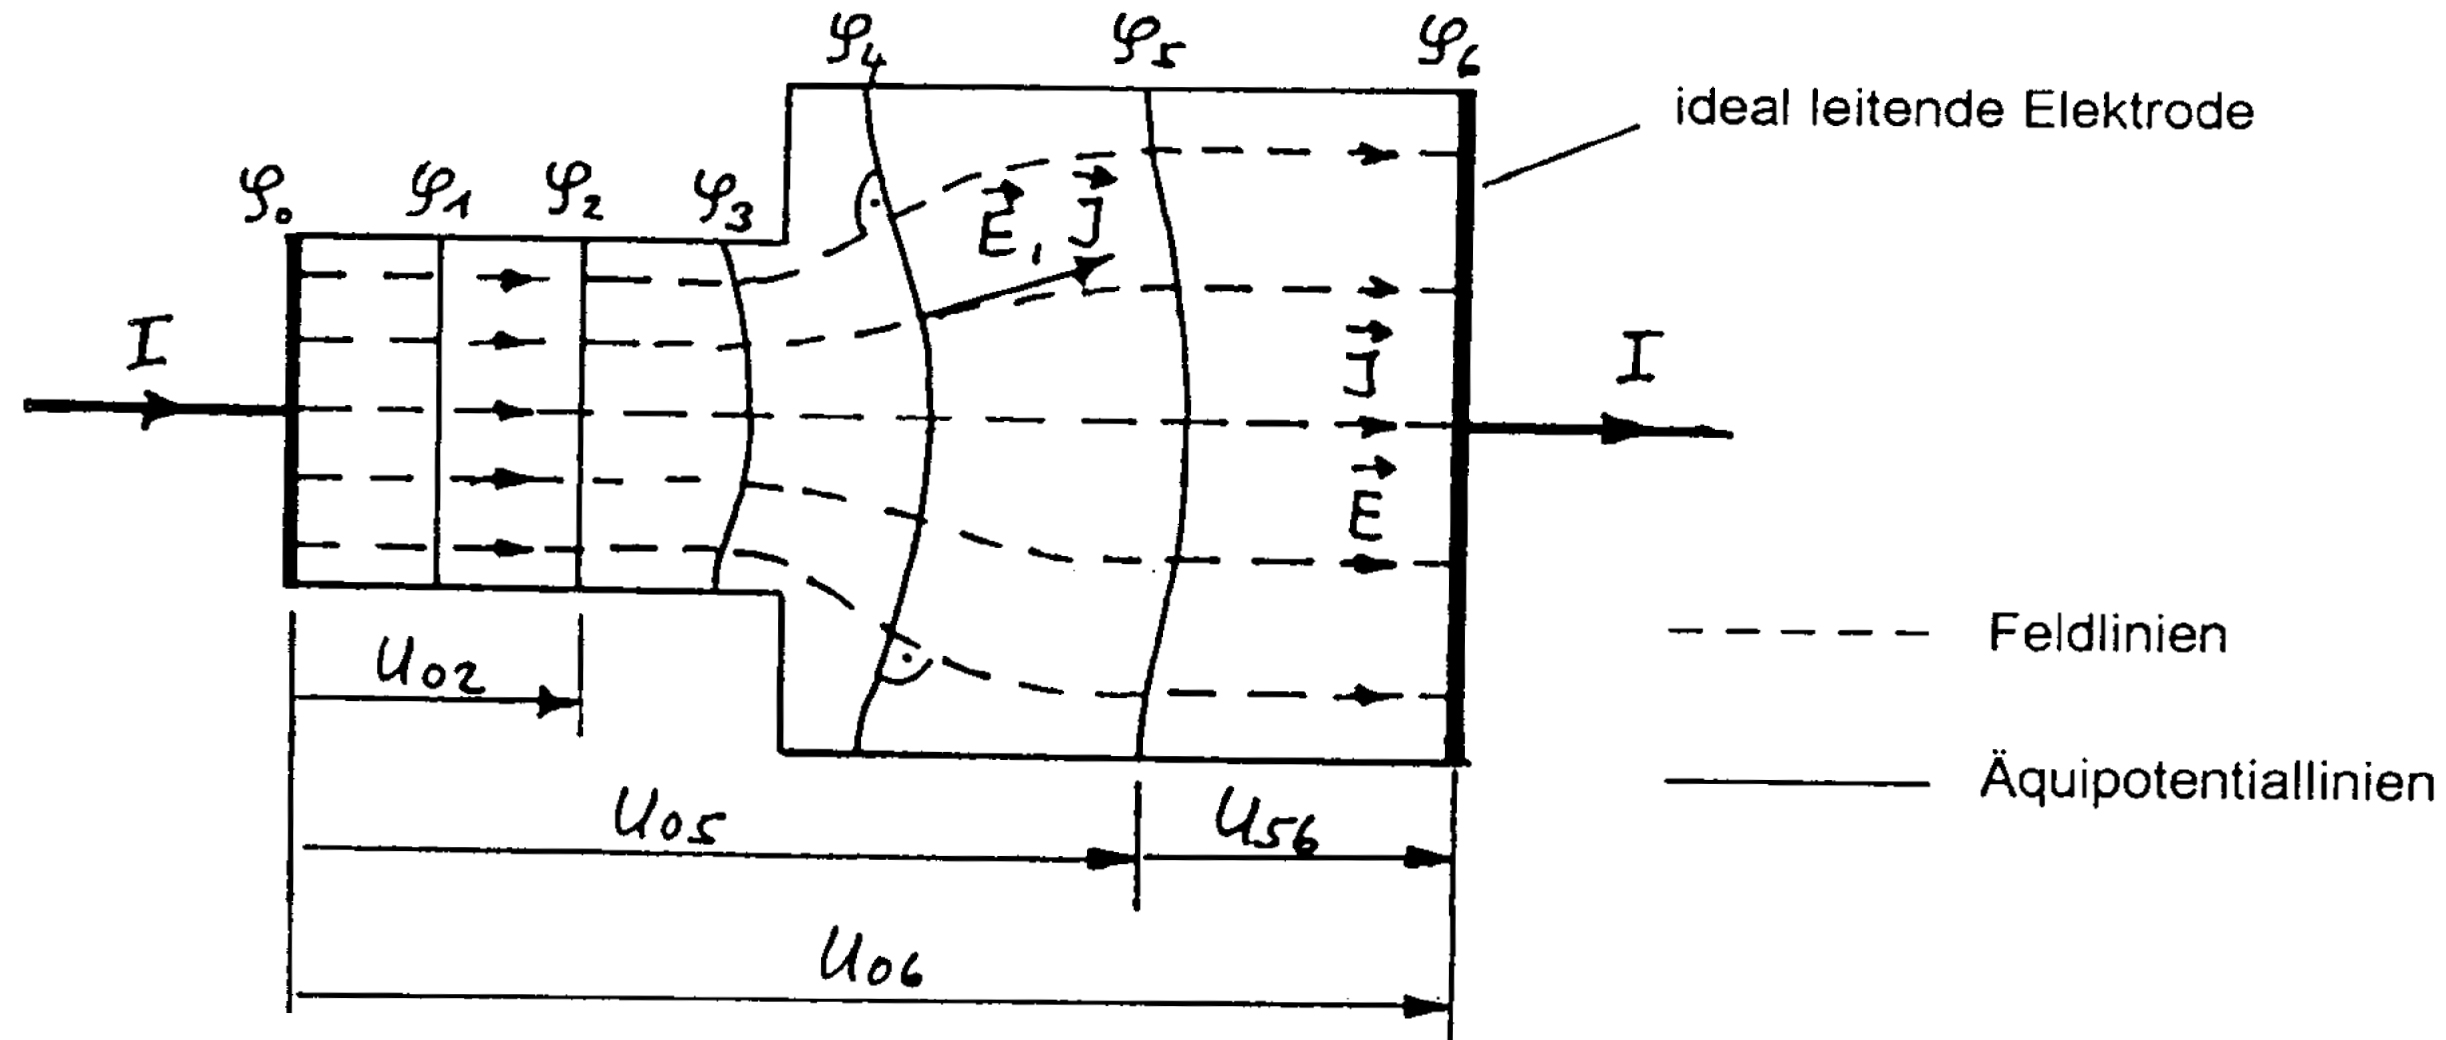
\includegraphics[width=0.4\textwidth]{pics/stroemungsfeld/feldlinien}\\
$ U_{AB} = \varphi_A - \varphi_B $\\
$ U_{AB} = \int\limits_{A}^B \vec E (s) \cdot  \vec{ds} $ \\
Im homogenen E Feld gilt zudem: \\
$ U_{AB} = E \cdot \overline{AB} \cdot \cos\alpha $ \\
\end{multicols}

\subsection{Kirchhoffsche Sätze im stationären Strömungsfeld}
Im stationären elektrischen Strömungsfeld ist der Strom durch eine beliebige in sich geschlossene Fläche ("`Hülle"') gleich null:\\
$ \int\limits_{H"ulle A} \vec J \cdot d \vec A = 0 $\\
Das Integral der elektrischen Feldstärke über einen beliebigen geschlossenen Weg ist gleich null:\\
$ \int \vec E \cdot d \vec s = 0 $\\

\subsection{Die Leistung im Str"omungsfeld}
$ \Delta{l} \ ist\ in\ $Strömungsrichtung,$\ \Delta{A} \ senkrecht\ dazu.$\\
$ \Delta P = \Delta U \cdot \Delta I $\\
$ Leistungsdichte\ p = \frac{\Delta P}{\Delta V} = \frac{\Delta U }{\Delta l} \cdot \frac{\Delta I}{\Delta A} = E \cdot J = \sigma E^2 = \rho \cdot J^2 $\\

\subsection{Vergleich Strömungsfeld - elektrostatisches Feld}
\begin{tabular}{ll}
Strömungsfeld & Elektrostatisches Feld\\
$ \vec{J} $ & $ \vec{D} $ (Flussdichte) \\
I & Q (Ladung)\\
$ \sigma $ & $ \varepsilon $ (Permittivität) \\

G & C (Kapazität) \\

Ohmsches Gesetz & Stoffgleichung \\

$ \vec J = \kappa \vec E $ & $ \vec D = \varepsilon \vec E $ \\

$ \vec E = \rho \vec J $ & $ \vec E = \frac{1}{\varepsilon} \vec D $ \\

J = Stromdichte & D = elektrische Flussdichte \\

$I = \int\limits_{A} \vec J d \vec A$ & $ \Psi_{el} = \int\limits_{A} \vec D d \vec A $ \\

Kirchhoff'sches Stromgesetz$ \int\limits_{H"ulle} \vec J d \vec A = 0$ & Quellengleichung $ \int\limits_{H"ulle} \vec D d \vec A = \sum Q_{eingeschl.}$\\

\multicolumn{2}{c}{Spannung, Potentialdifferenz A $\rightarrow$ B  $U_{AB} \int\limits_{A}^B \vec E \vec{ds}$} \\

\multicolumn{2}{c}{Potentialfeld: Kirchhoffsches Spannungsgesetz $\int \vec E \vec{ds} = 0 $} \\

Leitwert, Widerstand $ G = \frac{1}{R} = \frac{I}{U} $ & Kapazität $ C = \frac{\psi_{el}}{U} = \frac{Q}{U} $ \\

Räumliche Leistungsdichte $ p = E \cdot J = \kappa E^2 = \rho J^2 $ & Räumliche Energiedichte $ w = \frac{1}{2} D \cdot E = \frac{1}{2} \varepsilon E^2 $ \\
\end{tabular}

\subsection{Halbkugelerder}
\begin{multicols}{2}
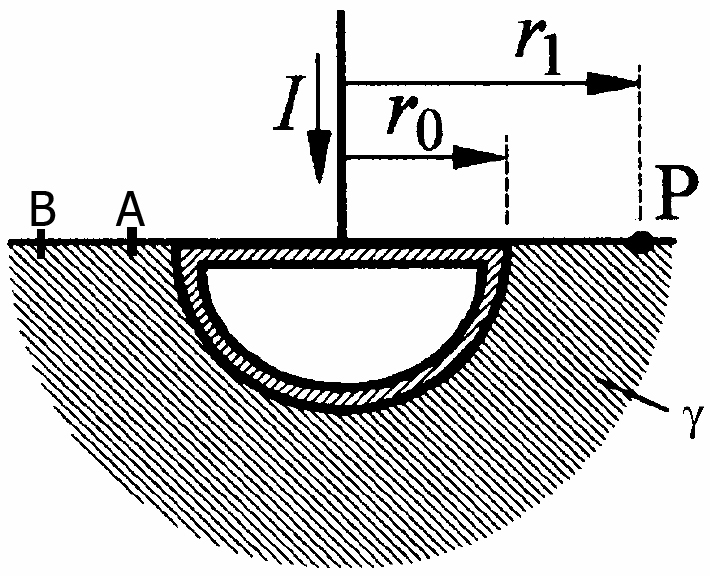
\includegraphics[width=0.3\textwidth]{pics/stroemungsfeld/halbkugelerder}\\
$ \varphi (r) = \int\limits_r^{\infty} E(r)\ dr = \frac{I}{2 \pi \sigma} \int\limits_r^{\infty} \frac{1}{r^2} dr = \frac{I}{2 \pi \sigma} \lbrack - \frac{1}{r} \rbrack_r^{\infty} = \frac{I}{2 \pi \sigma r}$ \\
$ U_P = \int\limits_{r_0}^{r_1} E(r)\ dr = \frac{I}{2 \pi \sigma}(-\frac{1}{r_1} + \frac{1}{r_0}) $\\
$ U_{AB} = \int\limits_{r_A}^{r_B} E(r)\ dr = \frac{I}{2 \pi \sigma}(-\frac{1}{r_B} + \frac{1}{r_A}) $ \\
Erdübergangswiderstand $ R = \frac{U}{I} = \frac{\varphi(r_0)}{I} $ \\
Widerstand zwischen A und B $ R_{AB} = \frac{r_B - r_A}{2 \pi \sigma r_A r_B} $ \\
Leistung die im Erdreich verloren geht: $ P = U \cdot I $ oder $ P = R \cdot I^2$ \\
\end{multicols}

\subsection{Strömungsfelder}
\begin{tabular}{ll|l}
& Räumliches Zentralfeld & Zylindrisches Koaxialfeld\\
& 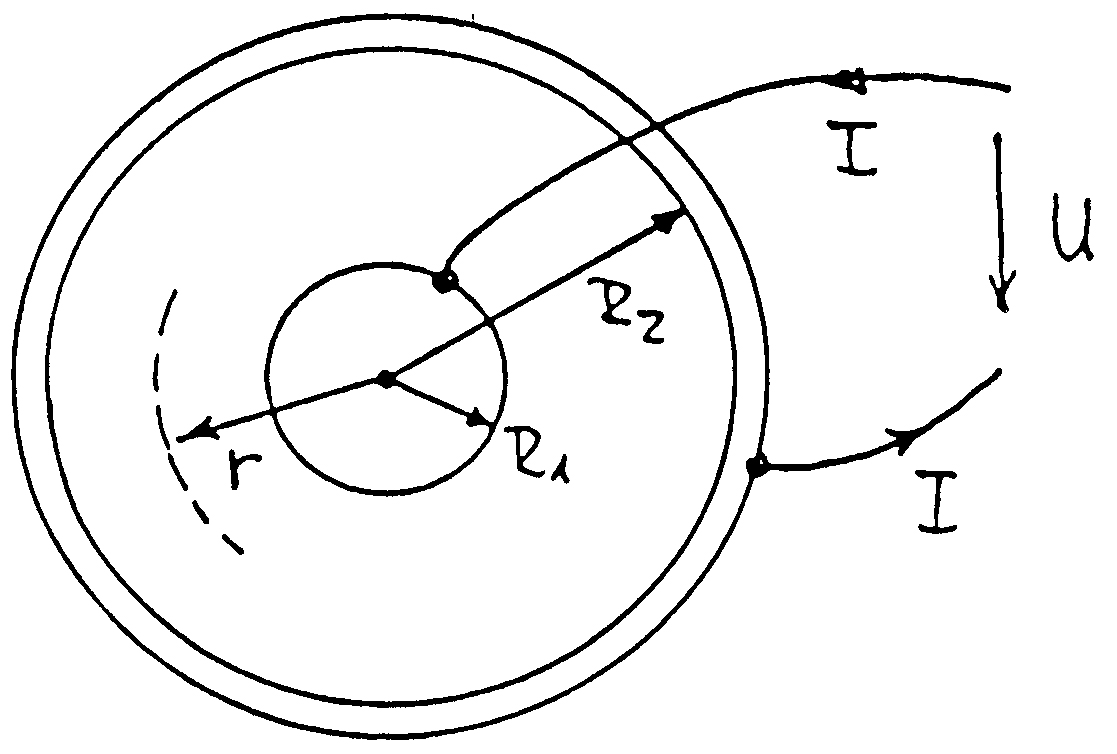
\includegraphics[width=0.2\textwidth]{pics/stroemungsfeld/zentralfeld}
& 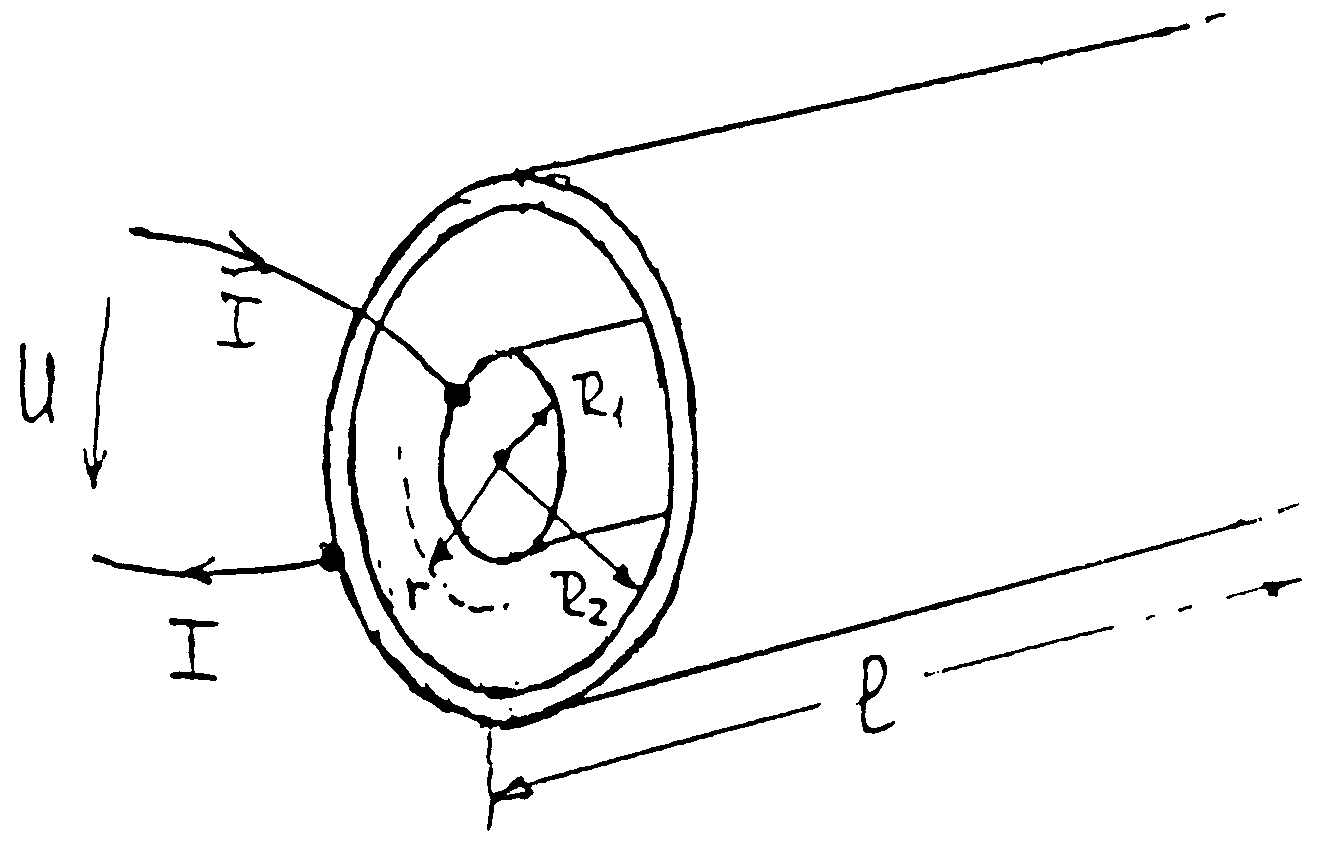
\includegraphics[width=0.2\textwidth]{pics/stroemungsfeld/koaxialfeld}\\
Hülle & $ A_{Kugel} = 4 \pi r^2 $ & $ A_{zyl} = 2 \pi r l $\\
Kirchhoff'sches Stromgesetz & $ J(r) \cdot 4 \pi r^2 - I = 0 $ & $ I - J(r) \cdot 2 \pi r l = 0 $ \\
Stromdichte & $ J(r) = \frac{I}{4 \pi r^2} $ & $ J(r) = \frac{I}{2 \pi r l} $ \\
Elektrische Feldstärke & $ E(r) = \frac{1}{\sigma} \cdot J(r) = \frac{I}{4 \pi \sigma r^2} $ & $ E(r) = \frac{J(r)}{\sigma} = \frac{I}{2 \pi l r \sigma} $ \\
Spannung & $ U = \int\limits_{R_{1}}^{R_{2}}E(r)\ dr = \frac{1}{4 \pi \sigma} \cdot \int\limits_{R_{1}}^{R_{2}}r^{-2}\ dr $ & $ U = \int\limits_{R_{1}}^{R_{2}}E(r)\ dr = \frac{I}{2 \pi l \sigma} \cdot \int\limits_{R_{1}}^{R_{2}}\frac{1}{r}\ dr $ \\
& $ = \frac{I}{4 \pi \sigma} (\frac{1}{R_{1}} - \frac{1}{R_{2}}) $ & $ = \frac{I}{2 \pi l \sigma} \cdot \ln \frac{R_2}{R_1}$ \\
\multicolumn{3}{l}{Potential $\varphi(r)$ "`Spannung gegenüber Bezugspunkt"'} \\
für $\varphi(R_1) = 0$ : & $ \varphi (r) = - \int\limits_{R_1}^rE(x)\ dx = - \frac{I}{4 \pi \sigma} (\frac{1}{R_1} - \frac{1}{r}) $ & $ \varphi (r) = \int\limits_{r}^{R_1}\vec{E}(r) \cdot \vec{dr} = -\int\limits_{R_1}^rE(r)\ dr = - \frac{I}{2 \pi l \sigma} \ln \frac{r}{R_1}$ \\
für $\varphi(R_2) = 0$ : & $ \varphi (r) = \int\limits_{r}^{R_{2}}E(x)\ dx = \frac{I}{4 \pi \sigma}(\frac{1}{r}-\frac{1}{R_2}) $ & $ \varphi (r) = \int\limits_{r}^{R_2}E(r)\ dr = \frac{I}{2 \pi l \sigma} \ln \frac{R_2}{r}$\\
Widerstand & $R = \frac{U}{I} = \frac{\frac{1}{R_1} - \frac{1}{R_2}}{4 \pi \sigma} = \frac{R_2 - R_1}{4 \pi \sigma \cdot R_1 \cdot R_2} $ & $R = \frac{U}{I} = \frac{\ln\frac{R_2}{R_1}}{2 \pi l \sigma} $ \\

\end{tabular}
